\chap{DEF-A30-X-5C}

\begin{table}[ht!]
    \centering
    \begin{tabular}{| p{2.0cm} | p{1.6cm} | p{1.6cm} | p{1.6cm} | p{1.6cm} | p{1.6cm} | p{1.6cm} | p{1.6cm} | p{2.0cm} | }
    \hline

	Expansion [\%] & 0-0.0001mm & 0.0001-0.001mm & 0.001-0.01mm & 0.01-0.1mm & 0.1+mm & Sum \\ \hline

    0.1671 &	586017 &	439450 &	36561 &	0 &	0 &	1062028\\ \hline
    0.3380 &	670005 &	616246 &	99949 &	5 &	0 &	1386205\\ \hline
    0.5118 &	708833 &	725962 &	155557 &	240 &	0 &	1590592\\ \hline
    0.8577 &	746251 &	853144 &	245537 &	3458 &	0 &	1848390\\ \hline

    \end{tabular}
    \caption{Number of Cracked Faces in Different Crack Width}
    \label{}
\end{table}


%% DEF_A30_X-5C_3 Internal Stress
\begin{figure}[ht!]
\centering
    %*******
    %*******
    \begin{subfigure}{.25\textwidth}
      \centering
      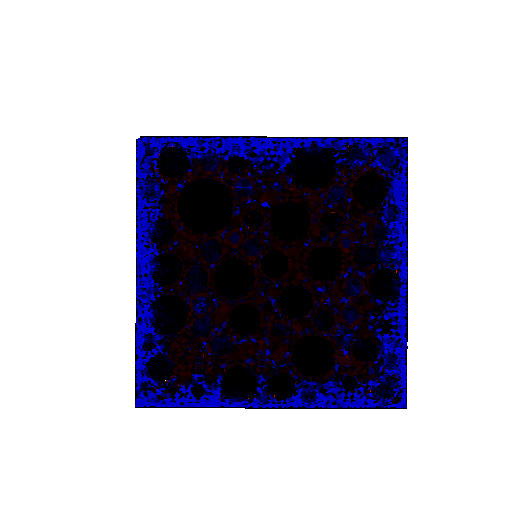
\includegraphics[width=1.0\linewidth]{Files/exp_3D/DEF/A30X-5C_1_s5.png}
      \caption{0.1671\% Expansion\\Internal Stress Step 5}
    \end{subfigure}%
    %*******
    \begin{subfigure}{.25\textwidth}
      \centering
      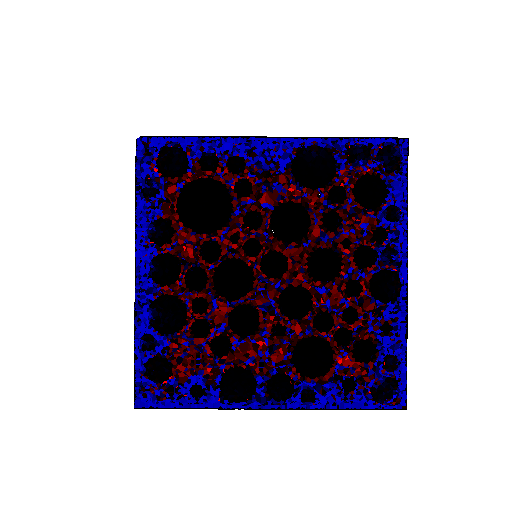
\includegraphics[width=1.0\linewidth]{Files/exp_3D/DEF/A30X-5C_1_s10.png}
      \caption{0.1671\% Expansion\\Internal Stress Step 10}
    \end{subfigure}%
    %*******
    \begin{subfigure}{.25\textwidth}
      \centering
      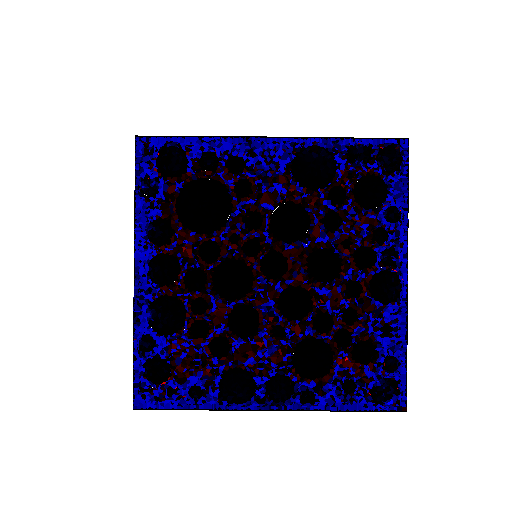
\includegraphics[width=1.0\linewidth]{Files/exp_3D/DEF/A30X-5C_1_s15.png}
      \caption{0.1671\% Expansion\\Internal Stress Step 15}
    \end{subfigure}%
    %*******
    \begin{subfigure}{.25\textwidth}
      \centering
      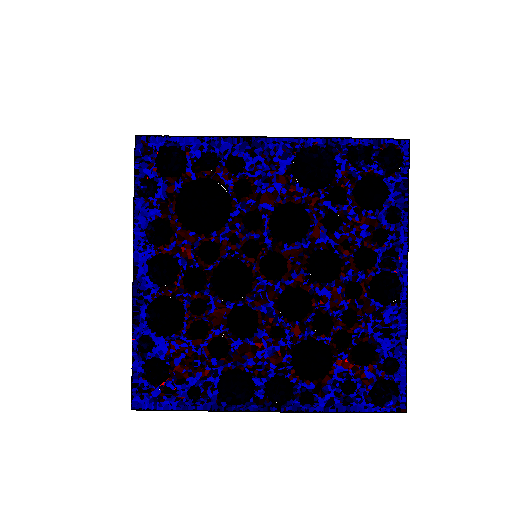
\includegraphics[width=1.0\linewidth]{Files/exp_3D/DEF/A30X-5C_1_stress.png}
      \caption{0.1671\% Expansion\\Internal Stress Step 20}
    \end{subfigure}
    %*******
    %*******
    \begin{subfigure}{.25\textwidth}
      \centering
      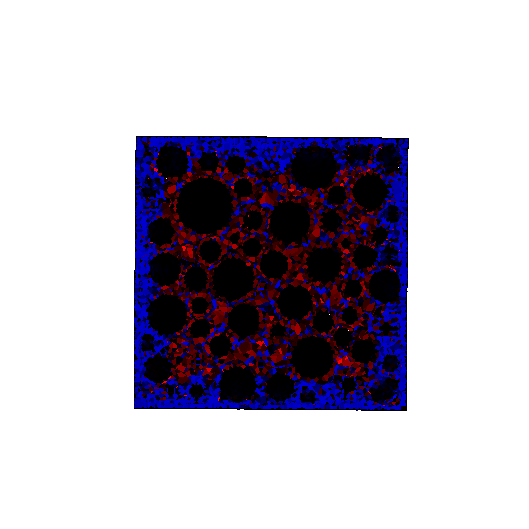
\includegraphics[width=1.0\linewidth]{Files/exp_3D/DEF/A30X-5C_2_s5.png}
      \caption{0.338\% Expansion\\Internal Stress Step 5}
    \end{subfigure}%
    %*******
    \begin{subfigure}{.25\textwidth}
      \centering
      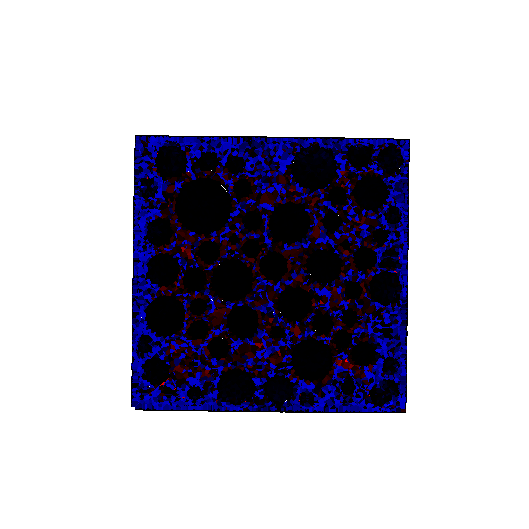
\includegraphics[width=1.0\linewidth]{Files/exp_3D/DEF/A30X-5C_2_s10.png}
      \caption{0.338\% Expansion\\Internal Stress Step 10}
    \end{subfigure}%
    %*******
    \begin{subfigure}{.25\textwidth}
      \centering
      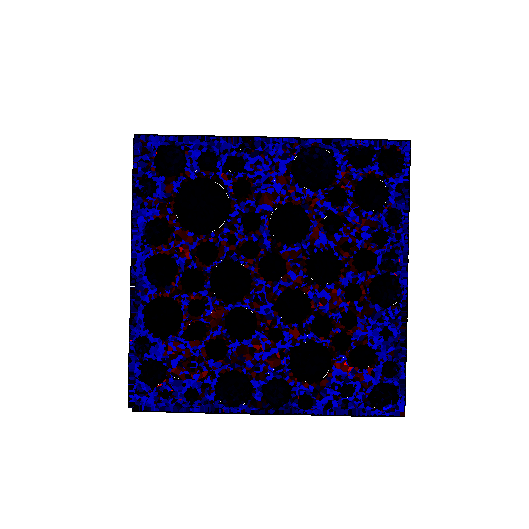
\includegraphics[width=1.0\linewidth]{Files/exp_3D/DEF/A30X-5C_2_s15.png}
      \caption{0.338\% Expansion\\Internal Stress Step 15}
    \end{subfigure}%
    %*******
    \begin{subfigure}{.25\textwidth}
      \centering
      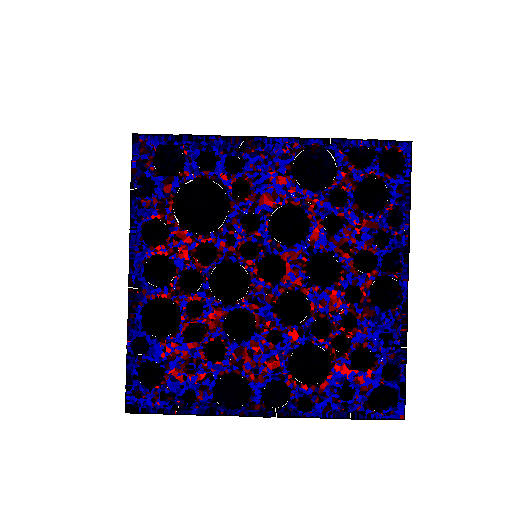
\includegraphics[width=1.0\linewidth]{Files/exp_3D/DEF/A30X-5C_2_stress.png}
      \caption{0.338\% Expansion\\Internal Stress Step 20}
    \end{subfigure}
    %*******
    %*******
    \begin{subfigure}{.25\textwidth}
      \centering
      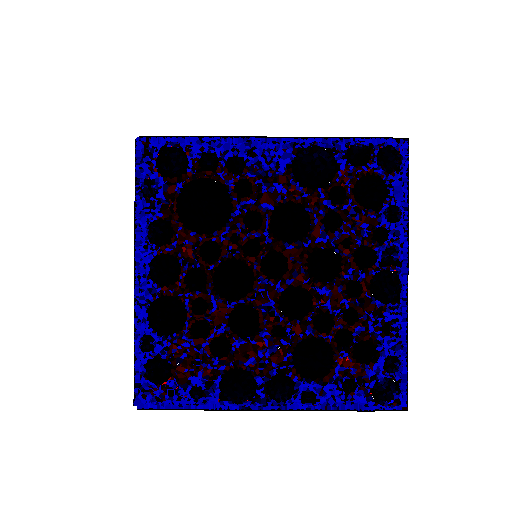
\includegraphics[width=1.0\linewidth]{Files/exp_3D/DEF/A30X-5C_3_s5.png}
      \caption{0.5118\% Expansion\\Internal Stress Step 5}
    \end{subfigure}%
    %*******
    \begin{subfigure}{.25\textwidth}
      \centering
      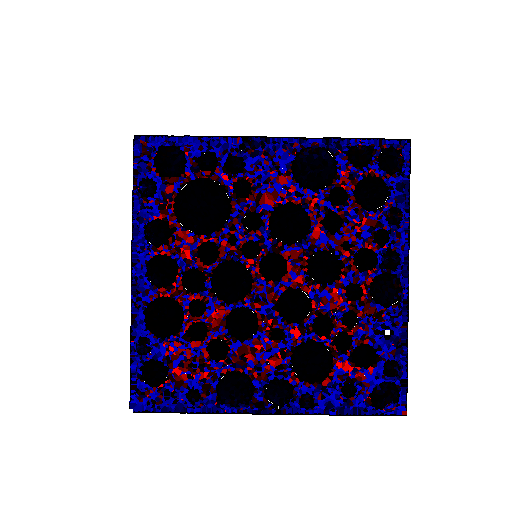
\includegraphics[width=1.0\linewidth]{Files/exp_3D/DEF/A30X-5C_3_s10.png}
      \caption{0.5118\% Expansion\\Internal Stress Step 10}
    \end{subfigure}%
    %*******
    \begin{subfigure}{.25\textwidth}
      \centering
      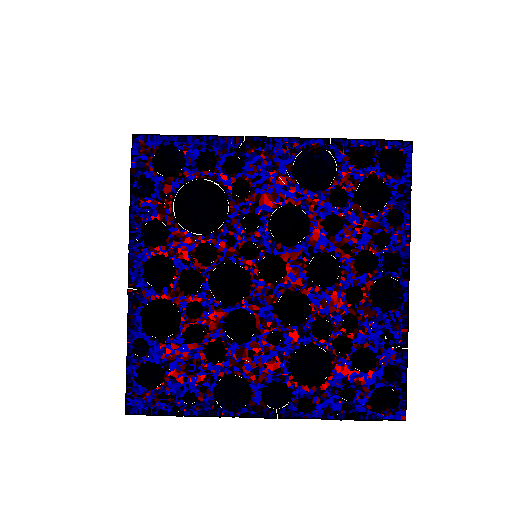
\includegraphics[width=1.0\linewidth]{Files/exp_3D/DEF/A30X-5C_3_s15.png}
      \caption{0.5118\% Expansion\\Internal Stress Step 15}
    \end{subfigure}%
    %*******
    \begin{subfigure}{.25\textwidth}
      \centering
      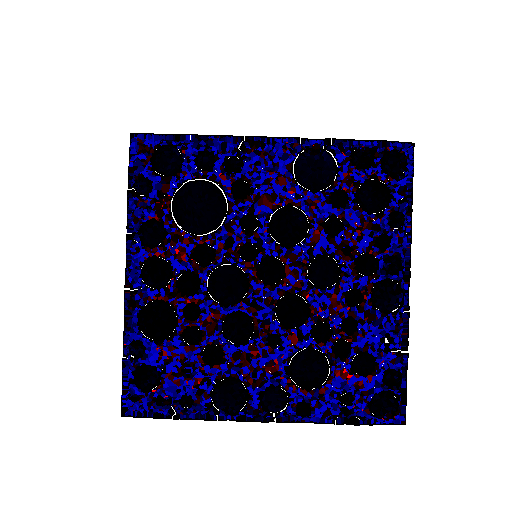
\includegraphics[width=1.0\linewidth]{Files/exp_3D/DEF/A30X-5C_3_stress.png}
      \caption{0.5118\% Expansion\\Internal Stress Step 20}
    \end{subfigure}
    %*******

    %*******
    \begin{subfigure}{.25\textwidth}
      \centering
      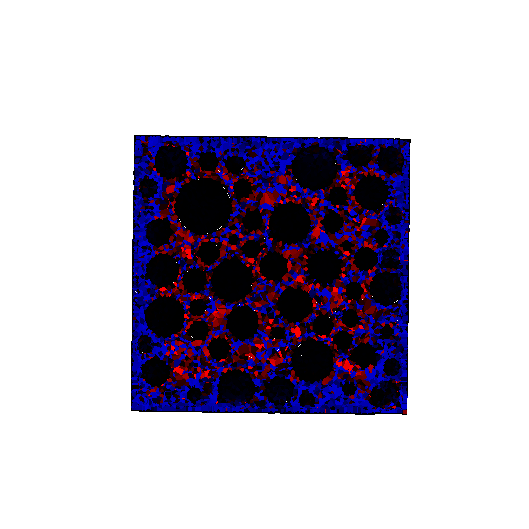
\includegraphics[width=1.0\linewidth]{Files/exp_3D/DEF/A30X-5C_4_s5.png}
      \caption{0.8577\% Expansion\\Internal Stress Step 5}
    \end{subfigure}%
    %*******
    \begin{subfigure}{.25\textwidth}
      \centering
      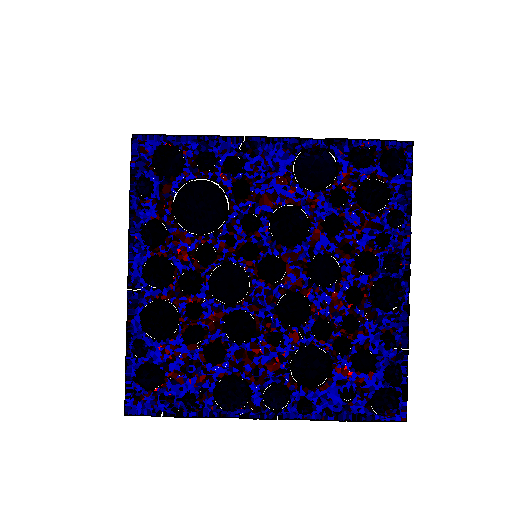
\includegraphics[width=1.0\linewidth]{Files/exp_3D/DEF/A30X-5C_4_s10.png}
      \caption{0.8577\% Expansion\\Internal Stress Step 10}
    \end{subfigure}%
    %*******
    \begin{subfigure}{.25\textwidth}
      \centering
      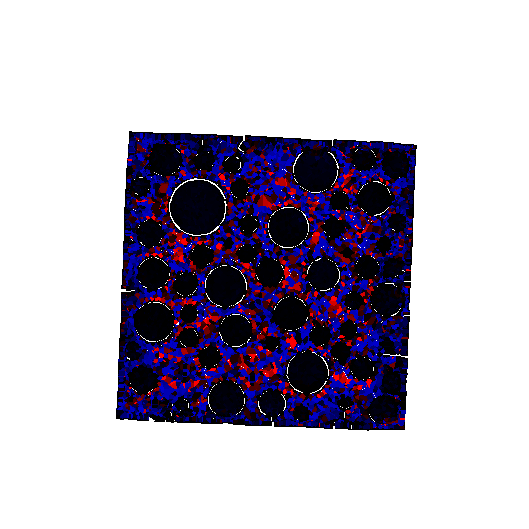
\includegraphics[width=1.0\linewidth]{Files/exp_3D/DEF/A30X-5C_4_s15.png}
      \caption{0.8577\% Expansion\\Internal Stress Step 15}
    \end{subfigure}%
    %*******
    \begin{subfigure}{.25\textwidth}
      \centering
      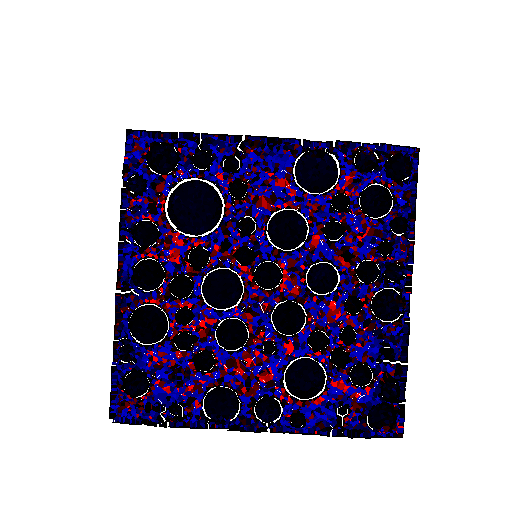
\includegraphics[width=1.0\linewidth]{Files/exp_3D/DEF/A30X-5C_4_stress.png}
      \caption{0.8577\% Expansion\\Internal Stress Step 20}
    \end{subfigure}
    %*******

\caption{Generation of Internal Stress for Expansion to Step 20(Final Expansion Step)}
\label{fig:A30_stress}
\end{figure}

\begin{figure}[ht!]
    \centering
    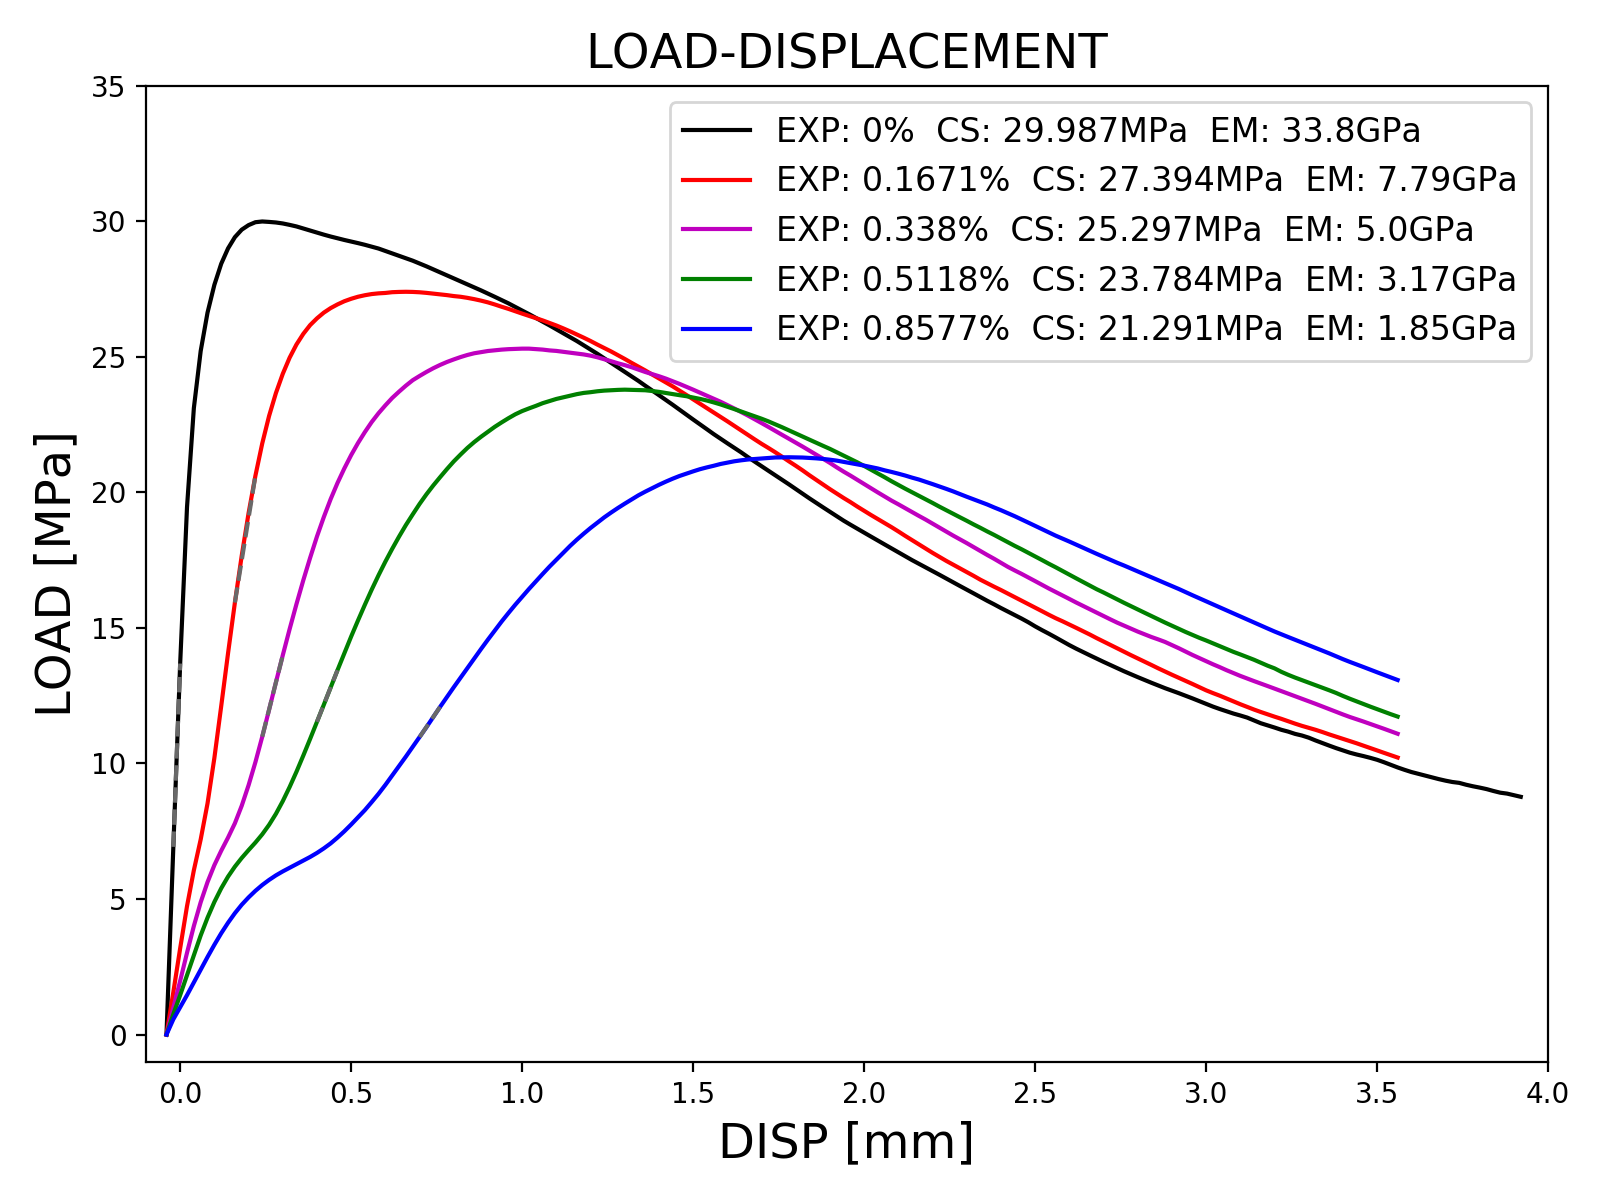
\includegraphics[width=0.8\linewidth]{Files/exp_3D/DEF/S13A30FIXX-5-LOAD-DISPLACEMENT.png}
    \caption{LOAD-DISPLACEMENT(Fix Boundary Condition)}
    \label{fig:S13A15FIXX-5-LOAD-DISPLACEMENT}
\end{figure}

%% DEF_A30_X-5C Surface Crack

\begin{figure}[ht!]
    \centering
    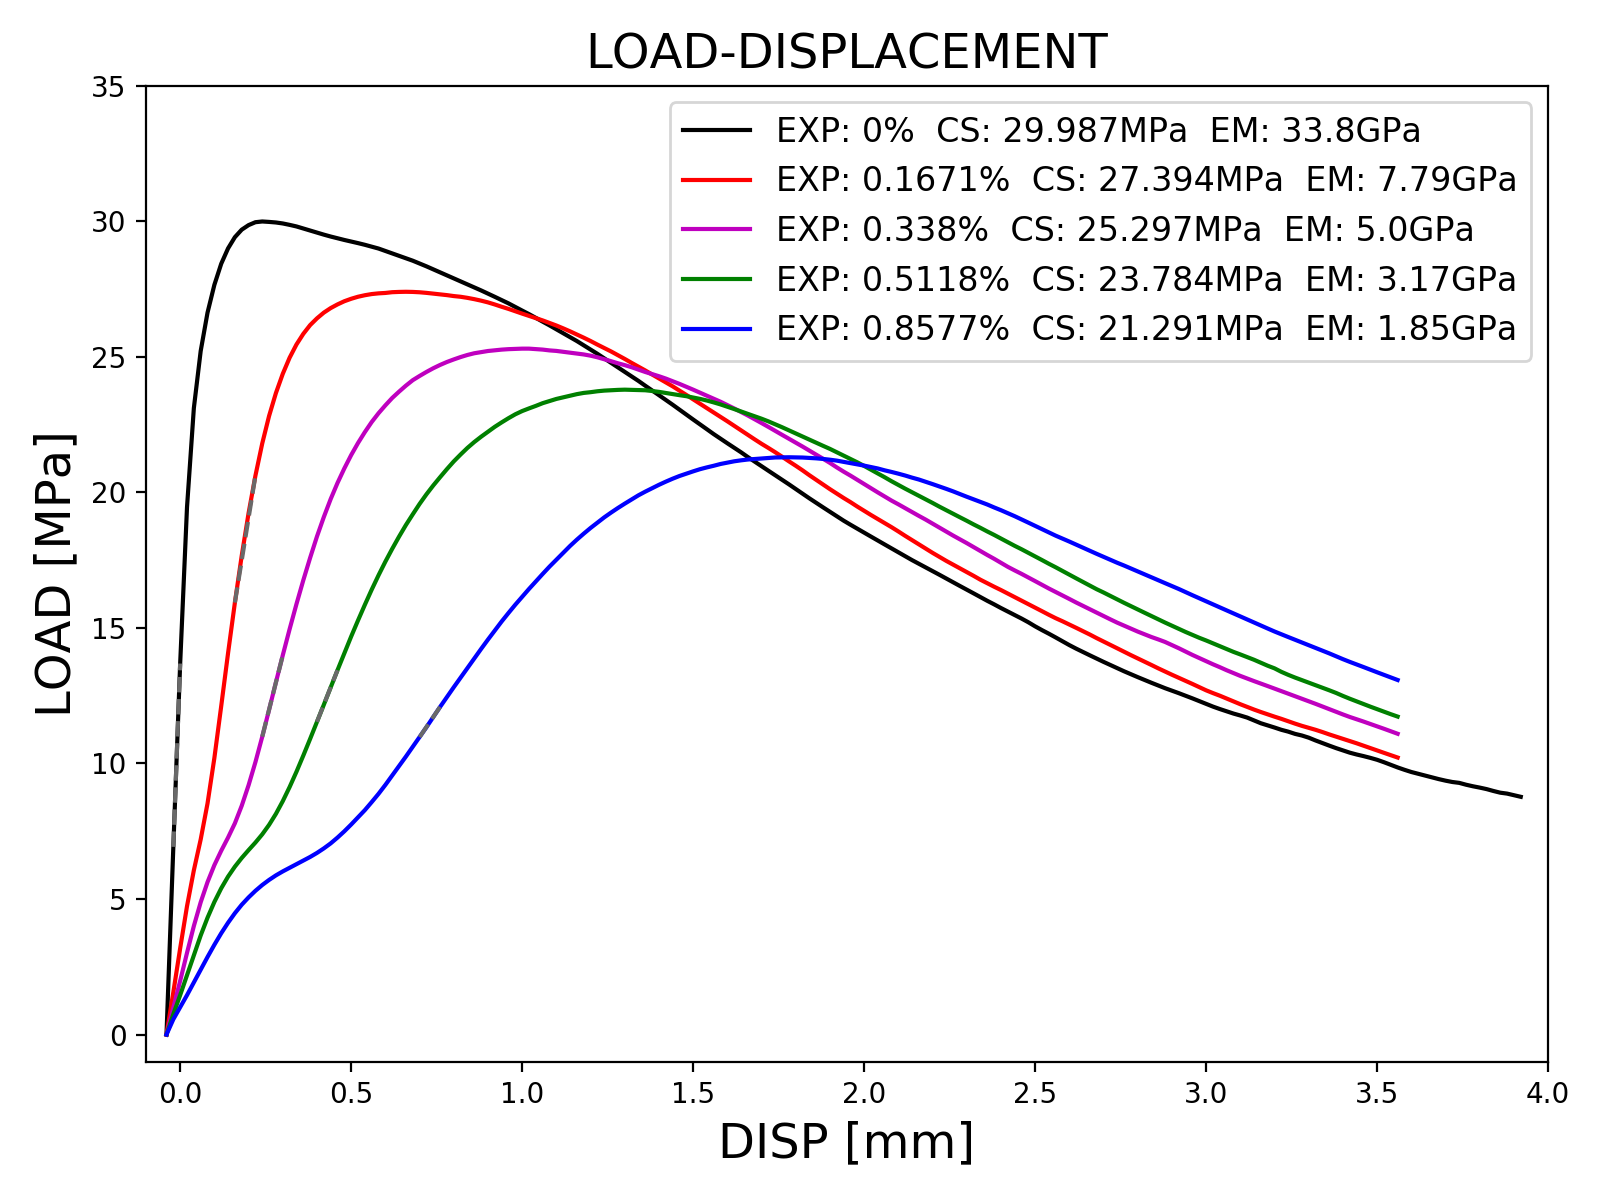
\includegraphics[width=0.8\linewidth]{Files/exp_3D/DEF/S13A30FIXX-5-LOAD-DISPLACEMENT.png}
    \caption{LOAD-DISPLACEMENT(Fix Boundary Condition)}
    \label{fig:S13A30X-5CFIX-LOAD-DISPLACEMENT}
\end{figure}

\begin{figure}[ht!]
\centering
    %*******
    %*******
    \begin{subfigure}{.5\textwidth}
      \centering
      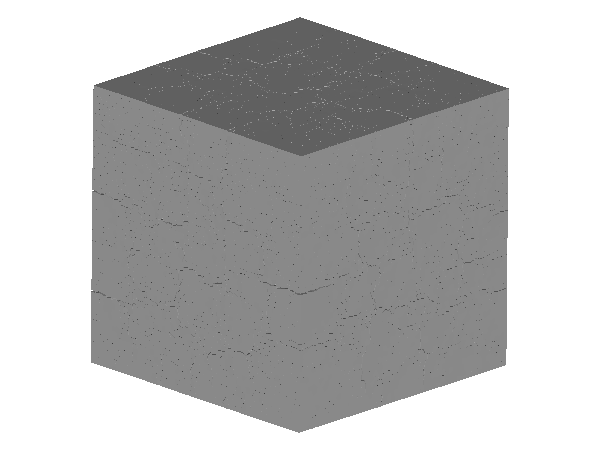
\includegraphics[width=0.5\linewidth]{Files/exp_3D/DEF/A30X-5C_1_3d.png}
      \caption{0.1671\% Expansion\\3D Surface Crack}
    \end{subfigure}%
    %*******
    \begin{subfigure}{.5\textwidth}
      \centering
      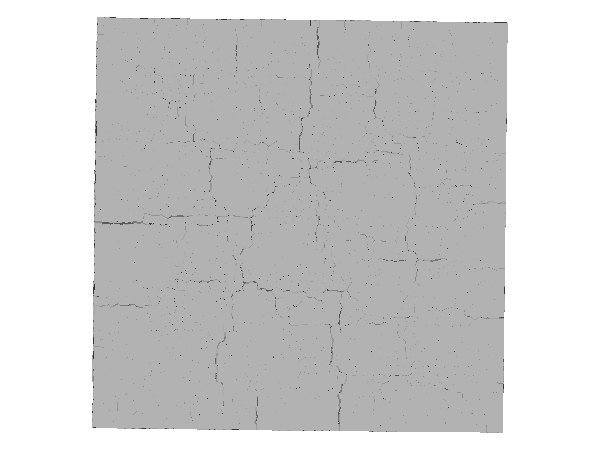
\includegraphics[width=0.5\linewidth]{Files/exp_3D/DEF/A30X-5C_1_3ds.png}
      \caption{0.1671\% Expansion\\3D Surface Crack (One Side)}
    \end{subfigure}%
    %*******

    %*******
    \begin{subfigure}{.5\textwidth}
      \centering
      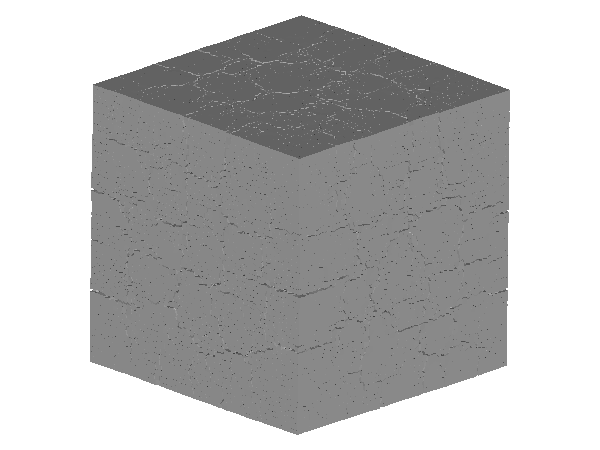
\includegraphics[width=0.5\linewidth]{Files/exp_3D/DEF/A30X-5C_2_3d.png}
      \caption{0.338\% Expansion\\3D Surface Crack}
    \end{subfigure}%
    %*******
    \begin{subfigure}{.5\textwidth}
      \centering
      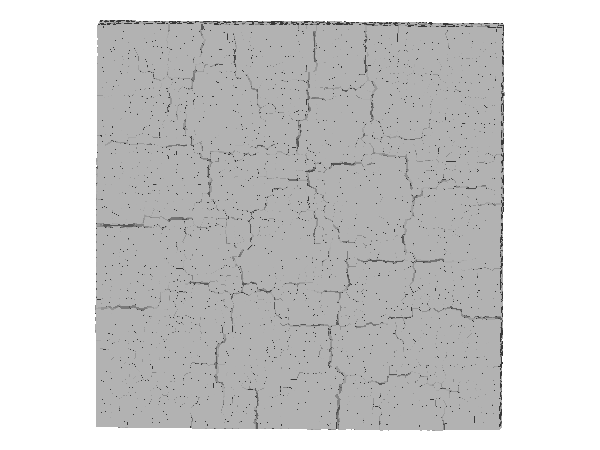
\includegraphics[width=0.5\linewidth]{Files/exp_3D/DEF/A30X-5C_2_3ds.png}
      \caption{0.338\% Expansion\\3D Surface Crack (One Side)}
    \end{subfigure}%
    %*******

    %*******
    \begin{subfigure}{.5\textwidth}
      \centering
      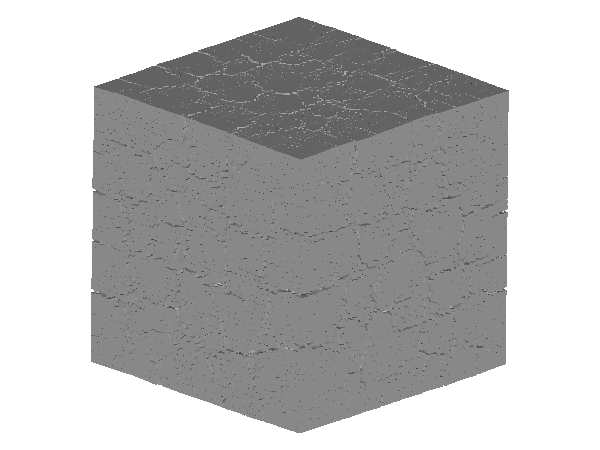
\includegraphics[width=0.5\linewidth]{Files/exp_3D/DEF/A30X-5C_3_3d.png}
      \caption{0.5118\% Expansion\\3D Surface Crack}
    \end{subfigure}%
    %*******
    \begin{subfigure}{.5\textwidth}
      \centering
      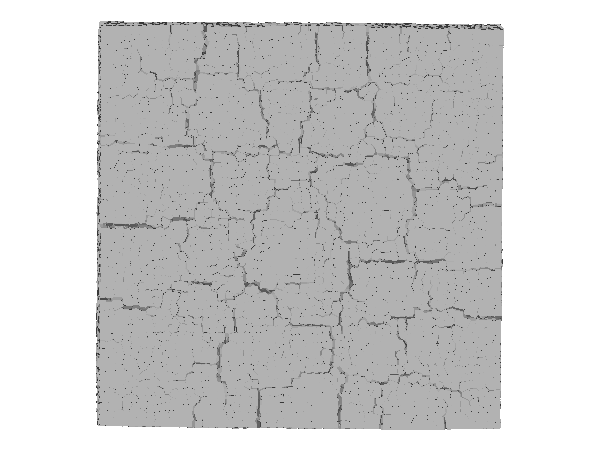
\includegraphics[width=0.5\linewidth]{Files/exp_3D/DEF/A30X-5C_3_3ds.png}
      \caption{0.5118\% Expansion\\3D Surface Crack (One Side)}
    \end{subfigure}%
    %*******

    %*******
    \begin{subfigure}{.5\textwidth}
      \centering
      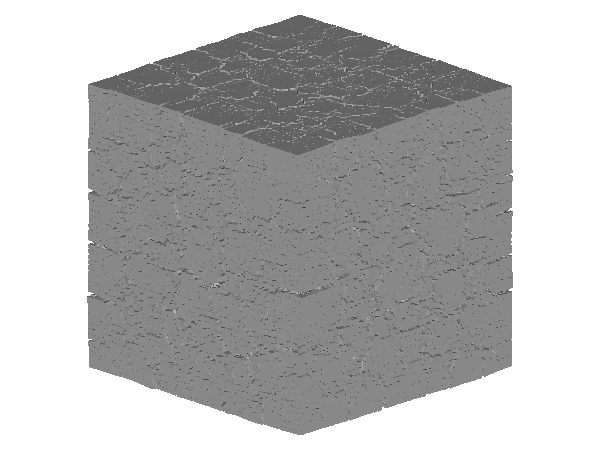
\includegraphics[width=0.5\linewidth]{Files/exp_3D/DEF/A30X-5C_4_3d.png}
      \caption{0.8577\% Expansion\\3D Surface Crack}
    \end{subfigure}%
    %*******
    \begin{subfigure}{.5\textwidth}
      \centering
      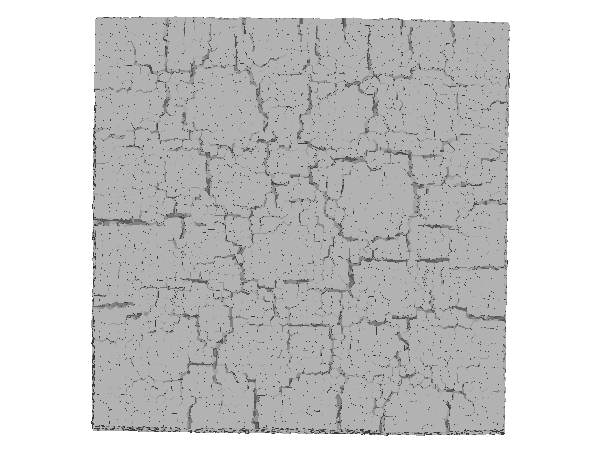
\includegraphics[width=0.5\linewidth]{Files/exp_3D/DEF/A30X-5C_4_3ds.png}
      \caption{0.8577\% Expansion\\3D Surface Crack (One Side)}
    \end{subfigure}%
    %*******

\caption{3D Surface Cracking Pattern}
\label{fig:A30_3Dcrack}
\end{figure}

\begin{figure}[ht!]
\centering
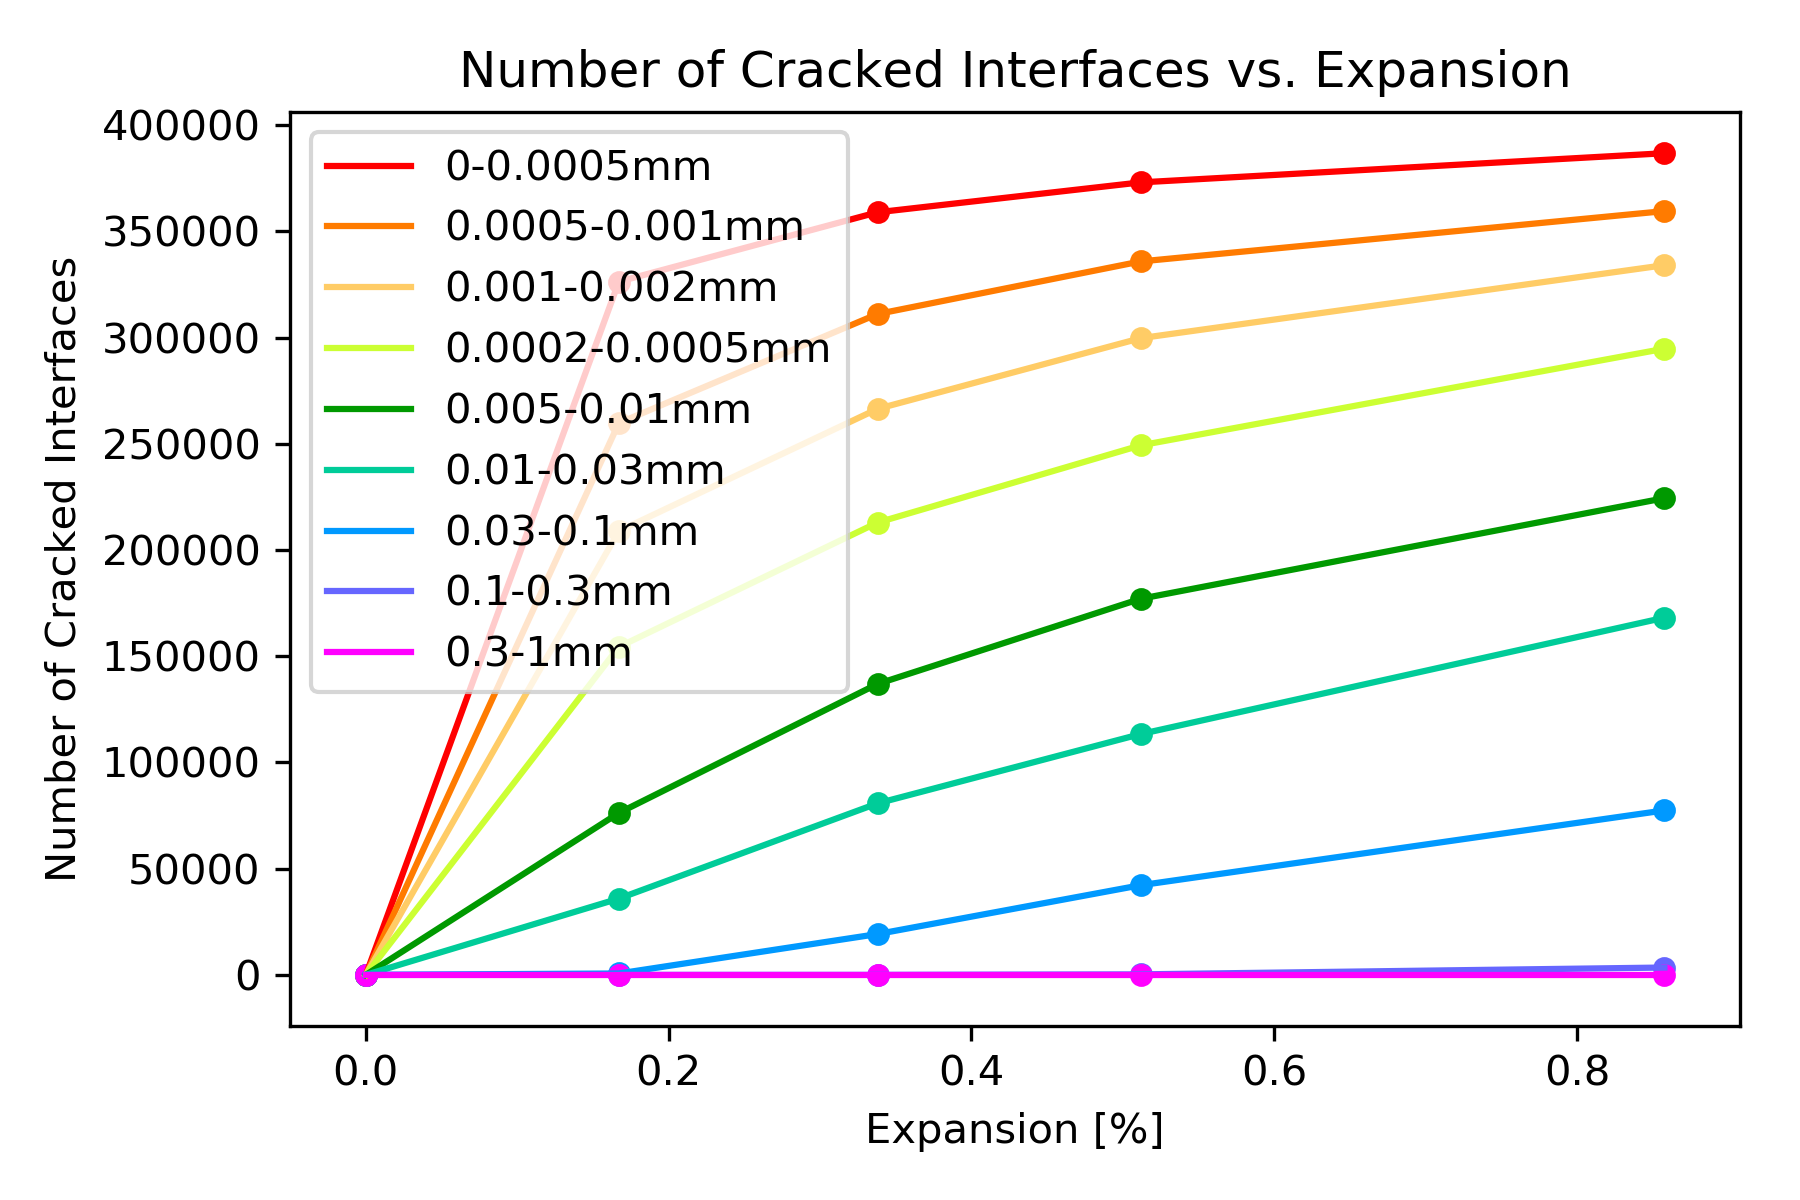
\includegraphics[width=.8\linewidth]{Files/interface/A30X-5CCRACK.png}
  \caption{Number of Cracked Interface vs. Expansion}
  \label{A30X-5CCRACK}
\end{figure}
